\section{Imaging and Image Processing}

Considering prediction of brain activity requires that we look not only at the
current state of brain simulation, but also towards the future. A Biological
brain processing the life of an organism, and a simulation of the same requires
a link to made between the two: the state of the brain must be copied over as a
snapshot. This imaging process would likely take the form of an in-vitro scan of
a preserved nervous system or some form of in-vivo scan. These images would be
processed and turned into a model that could be simulated. Current techniques for imaging the brain give us some insight to how this
uploading process might function and perform.

\subsection{Current Methods of Scanning the brain}

Given a 2D substrate such as a layer of brain
tissue, there are several methods of producing a high resolution image. These
methods typically balance the required resolution and image noise with the speed
and scale with which the image is created.

\begin{figure}[h]
    \centering
    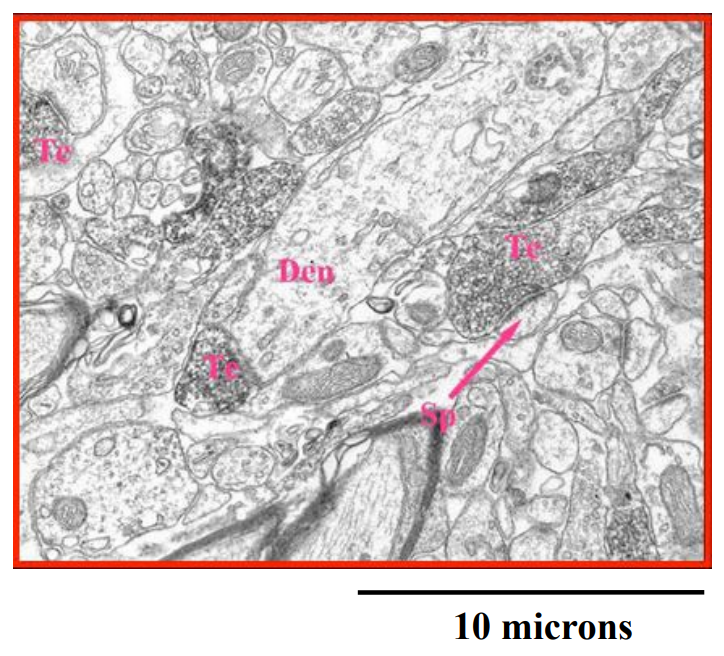
\includegraphics{figures/graphs/scaleexample.png}
    \DoubleCaption{Image depicting the scale of the the brain.}
    {TEMPORARY IMAGE}
    \label{scaleexample}
\end{figure}
\vspace{1ex}

Given the level of emulation that is intended from a model, the images that
synthesise the model must resolve a minimum level of detail. In figure
\ref{scaleexample}, the general position of axons(??) and rough links between
them can be identified, but more subtle morphologies of these links are missing.
Another imaging method could resolve further detail and allow for such
morphologies to be processed by a simulation. The specifications and drawbacks
of such imaging methods are described below.

\subsubsection*{MRI Scanning}

- Common procedure
- Enough detail for general structure, but provides little to no insight to fine
details such as placement of dendritic!Typo?! spines or the exact size or placement of
synapses between neurons.
- As the patient is typically alive during a scan, there will be significant
measurement drift as the current is still moving around the brain as normal.

\subsubsection*{XRay}

- Not naturally useful, have to inject a substrate into the brain for this to
create an image of any meaningful contrast ?!?!CITE
- Variants exist which provide much higher resolution but at the cost of time 

\subsubsection*{Electron Microscope Scanning}

- Very precise
- Can take a very long time
- Need well "frozen" slices of the brain for this to be of any use or you'll
have major measurement drift as the brain decays.

\subsection{Turning image data into a connectome}

\begin{quote}
    Dense connectomic mapping of neuronal circuits is limited by the time and
    effort required to analyze 3D electron microscopy (EM) datasets. Algorithms
    designed to automate image segmentation suffer from substantial error rates
    and require significant manual error correction. Any improvement in
    segmentation error rates would therefore directly reduce the time required
    to analyze 3D EM data.
    \autocite{pallotto_extracellular_2015} 

    The delineation of morphologies has proven to be the most difficult step to
    automate. Current machine learning-based analysis methods enable
    semi-automated reconstructions (segmentations) of neurons that still require
    significant human effort to correct.
    \autocite{helmstaedter_connectomic_2013}
\end{quote}

\subsection[Error induced through noise]{Examination of Error induced through the imaging process}

Prediction of future brain activity through simulation requires an accurate and
detailed connectome of a brain, with synapses and neurons correctly located in
space.\autocite{bostrom_whole_2008} The accuracy of such a model depends on the
resolution of the imaging method used to create it. The error resulting from
such a imaging method is the measurement error. Depending on imaging procedure, brain matter may shift in composition during the course of the scan, which is the cause of measurement drift, itself a form of measurement error.

\setlength{\tabcolsep}{4ex}
\renewcommand{\arraystretch}{1.1}
\begin{table}[ht]
    \centering
    \begin{tabular}{@{}llll@{}}
        Method              & Resolution                 & Time    & Error(approx.) \\
        \hline
        MRI                 & 6$\mu m$                   & 30mins  & 95\%           \\
        MRI microscopy      & 3$\mu m$                   & -       & 85\%           \\
        XRay microscopy     & 30nm                       & -       & 30\%           \\
        Electron microscopy & \textasciitilde 30nm-0.1nm & >3mnths & <1\%           \\
        Theoretical Ideal   & <5nm                       & <500s   & <1\%           \\
        \hline
    \end{tabular}
    \DoubleCaption{Comparison of imaging methods.}{Error approximated from size of dendritic spines.}
    \label{imagemethodcomparison1}
\end{table}
\setlength{\tabcolsep}{1ex}

